\begin{enumerate}
	\item In an equilateral $\triangle$ ABC, D is a point on side BC such that $ BD =\frac{1}{3}BC$. Prove that $9(AD)^2 = 7(AB)^2$.
	\hfill\brak{10, 2018}\item Prove that, in a right triangle, the  square on the hypotenuse is equal to sum of the squares on the other two sides.
	\hfill\brak{10, 2018}\item Prove that the area of an equilateral triangle described on one side of the square is equal to half of the area of the equilateral triangle described on one of its diagonal.
	\hfill\brak{10, 2018}\item If the area of two similar triangles are equal, prove that they are congruent.
\hfill\brak{10, 2018}
\item In figure,\figref{fig:rightangled4} BN and CM are medians of a $\triangle$ ABC right-angled at A. Prove that \begin{align}4(BN^2 +CM^2) = 5BC^2\end{align} 
\begin{figure}[!ht]
\centering
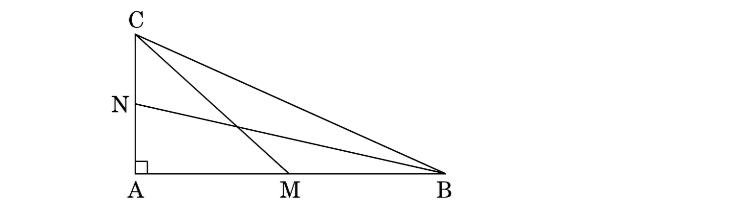
\includegraphics[width=\columnwidth]{cbse-math/figs/rightangled}
\caption{Right-angled triangle}
\label{fig:rightangled4}
\end{figure}

\hfill\brak{10, 2022}\item $\vec{Case Study - 1:}$
\begin{center}
$\vec{Kite Festival}$\\
\end{center}
Kite festival is celebrated in many countries at different times of the year. in India, every year 14th
January is celebrated as international kite Day. on his day many people visit India and participate in the festival by flying various kinds of kites.
\\The picture given below \figref{fig:kites5} , three kites flying together.
\begin{figure}[!ht]
\centering
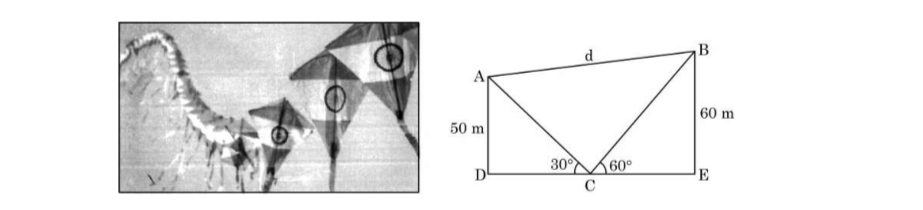
\includegraphics[width=\columnwidth]{cbse-math/figs/kites}
\caption{kites flying to gether}
\label{fig:kites5}
\end{figure}
\\In \figref{fig:kites5}, the angles of elevation of two kites (point C) are found to be $\degree{30}$ and  $\degree{60}$ respectively. Taking \begin{align}AD = 50 m\end{align} and\begin{align} BE = 60 m\end{align}
find
\begin{enumerate}
\item The length of string used (take them straight) for kites A and B as shown in the figure.
\item The distance 'd' between these two kites
\end{enumerate}
\hfill\brak{10, 2022}
\item Simplest form of 
 \begin{align}
     \frac{1 + \tan^{2}{A}}{1 + \cot^{2}{A}}
 \end{align}is .

\hfill\brak{10, 2020}\item Write the value of
 \begin{align}
	     \sin^{2}{30\degree} + \cos^{2}{60\degree}
	\end{align}.
\hfill\brak{10, 2020}\item If $A$, $B$ and $C$ are interior angles of $ \triangle ABC$, then show that
	\begin{align}
	    \cos \brak{\frac{B + C}{2}}=\sin \brak{\frac{A}{2}}
	\end{align}
      
\hfill\brak{10, 2020}\item Prove that : 
        \begin{align}
           (\sin^{4}{\theta} - \cos^{4}{\theta} + 1)\csc^{2}{\theta} = 2 
        \end{align}
\hfill\brak{10, 2020}
\item
If
\begin{align}
\cos\brak{\sin^{-1}{\frac{2}{\sqrt{5}}} + \cos^{-1}{x}} = 0
\end{align}
then $x$ is equal to
		\begin{multicols}{4}
\begin{enumerate}
	\item $\frac{1}{\sqrt{5}}$
	\item $-\frac{2}{\sqrt{5}}$
	\item $\frac{2}{\sqrt{5}}$
        \item $1$
\end{enumerate}
		\end{multicols}
\hfill\brak{12, 2020}
\item prove that \begin{align} \frac{\sin A-2 \sin^3A}{2\cos^3A-\cos A}=\tan A\end{align} 
  \hfill\brak{10, 2023}\item \begin{align} \sec A (1-\sin A)(\sec A+\tan A)=1\end{align} 

\hfill\brak{10, 2023}\item If 
\begin{align}
    4\cot^2 45\degree - \sec^2 60\degree + \sin^2 60\degree + p = \frac{3}{4}, 
\end{align}
then find the value of $p$.
\hfill\brak{10, 2023}\item If 
\begin{align}
    \cos A+ \cos^2A=1,
\end{align}then find the value of 
\begin{align}
\sin^2A+\sin^4A.
\end{align}
\hfill\brak{10, 2023}\item Prove that:\\
\begin{align}
\brak{\frac{1}{\cos\theta}-\cos\theta}\brak{\frac{1}{\sin\theta}-\sin\theta} = \frac{1}{\tan\theta+\cot\theta}
\end{align}




\hfill\brak{10, 2023}\item If $2\tan A=3$, then the value of $\frac{4sin A + 3\cos A}{4\sin A - 3\cos A}$ is
\begin{enumerate}
\item $\frac{7}{\sqrt{13}}$
\item $\frac{1}{\sqrt{13}}$
\item $3$
\item does not exist
\end{enumerate}



    \hfill\brak{10, 2023}\item $\brak{\sec^2\theta - 1}\brak{\csc^2\theta - 1}$  is equal to:
    \begin{enumerate}
   \item $-1$
   \item  $1$
   \item  $0$
   \item  $2$
        \end{enumerate}
   \hfill\brak{10, 2023}\item Evaluate $2\sec^2\theta+3\csc^2\theta-2\sin\theta\cos\theta$ if
   \begin{align}
      \theta=45\degree
   \end{align}
   
   \hfill\brak{10, 2023}\item If
   \begin{align}
       \sin\theta-\cos\theta=0
   \end{align}
   ,then find the value of $\sin^4\theta+\cos^4\theta$.
  \hfill\brak{10, 2023}
    \item If $\sin \theta=0$, then the value of $\tan^2\theta+\cot^2\theta$ is
    \begin{enumerate}
        \item $2$
        \item $4$
        \item $1$
        \item $\frac{10}{9}$
    \end{enumerate}
    \hfill\brak{10, 2022}\item $5\tan^2 \theta - 5\sec^2\theta = \underline{\hspace{2cm}}$
    \hfill\brak{10, 2022}\item In  \figref{fig:as.jpeg}, a tower stands vertically on the ground. From a point on the ground, which is $80m$ away from the foot of the tower, the angle of elevation of the tower is found to be $30\degree$. Find the height of the tower.
    \begin{figure}[H]
        \centering
        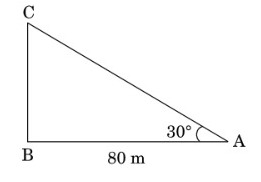
\includegraphics[width=70mm]{cbse-math/figs/as.jpeg}
        \caption{as.jpeg}
        \label{fig:as.jpeg}
    \end{figure}
    \hfill\brak{10, 2022}\item Show that 
    \begin{align}
        \cos(38\degree) \cos(52\degree) - \sin(38\degree)\sin(52\degree) = \cos(90\degree).
    \end{align}
    \hfill\brak{10, 2022}\item Prove that 
    \begin{align}
        \frac{\sin\theta}{\cot\theta+\csc\theta} = 2+\frac{\sin\theta}{\cot\theta-\csc\theta}.
    \end{align}
    \hfill\brak{10, 2022}\item Given 
    \begin{align}
        15 \cot (A) = 8,
    \end{align}
    find the values of $\sin (A)$ and $\sec (A)$.
    \hfill\brak{10, 2022}\item The angles of depression of the top and bottom of a tower as seen from the top of a $60\sqrt{3}m$ high cliff are $45\degree$ and $60\degree$ respectively. Find the height of the tower. (Use $\sqrt{3}=1.73$)
    \hfill\brak{10, 2022}\item The angle of elevation of the top of a building from the foot of the tower is $30\degree$ and the angle of elevation of the top of the tower from the foot of the building is $60\degree$. If the tower is $50$ meters high, then find the height of the building.
    \hfill\brak{10, 2022}\item From a point on a bridge across a river, the angles of depression of the banks on opposite sides of the river are $30\degree$ and $60\degree$ respectively. If the bridge is at a height of $3$ meters from the banks, then find the width of the river. 
    \hfill\brak{10, 2022}\item In \figref{fig:ak}, Gadisar Lake is located in the Jaisalmer district of Rajasthan. It was built by the King of Jaisalmer and rebuilt by Gadsi Singh in the $14$th century. The lake has many Chhatris. One of them is shown below:
    \begin{figure}[H]
        \centering
    	 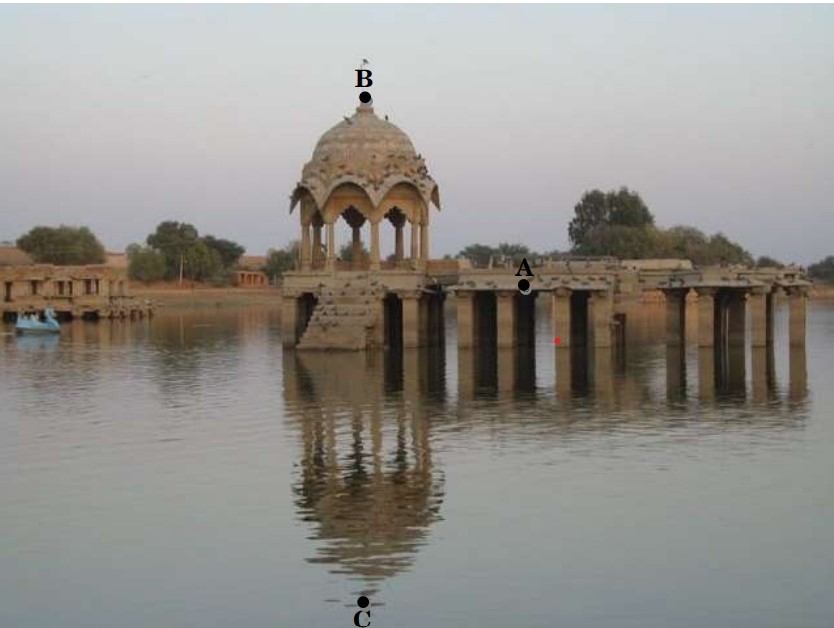
\includegraphics[width=70mm]{cbse-math/figs/ak.jpeg}
        \caption{ak.jpg}
        \label{fig:ak}
    \end{figure}
    Observe the picture. From a point $A$ $h$ meters above the water level, the angle of elevation of the top of Chhatri (point $B$) is $45\degree$ and the angle of depression of its reflection in the water (point $C$) is $60\degree$ . If the height of Chhatri above water level is (approximately) $10$ meters, then 
    \begin{enumerate}
        \item Draw a well-labeled figure based on the above information.
        \item Find the height ($h$) of the point $A$ above water level. (Use $\sqrt{3}=1.73$) 
    \end{enumerate}

    \hfill\brak{10, 2022}\item In \figref{fig:su.jpeg}, from a point on a bridge across a river, the angles of depression of the banks on opposite sides of the river are $30\degree$ and $45\degree$. If the bridge is at a height of $8$ meters from the banks, then find the width of the river.
    \begin{figure}[H]
        \centering
        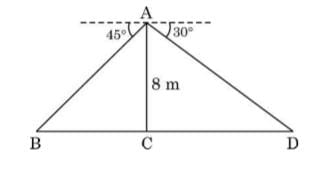
\includegraphics[width=70mm]{cbse-math/figs/su.jpeg}
        \caption{su.jpg}
        \label{fig:su.jpeg}
    \end{figure}
    
    \hfill\brak{10, 2022}\item Case Study-1:
    
    In \figref{fig:kite.jpeg}, Kite Festival is celebrated in many countries at different times of the year. In India, every year on $14^{th}$ January is celebrated as International Kite Day. On this day, many people visit India and participate in the festival by flying various kinds of kites.
    
    \begin{figure}[H]
	\centering
        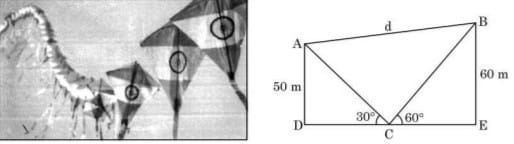
\includegraphics[width=70mm]{cbse-math/figs/kite.jpeg}
        \caption{kites}
        \label{fig:kite.jpeg}
    \end{figure}
    
    In Fig. 5, the angles of elevation of two kites (Point $A$ and $B$) from the hands of a man (Point $C$) are found to be $30\degree$ and $60\degree$ respectively. Taking $AD = 50$ meters and $BE = 60$ meters, find:
    \begin{enumerate}
        \item The lengths of strings used (take them straight) for kites $A$ and $B$ as shown in the figure.
        \item The distance $d$ between these two kites.
    \end{enumerate}
    
    \hfill\brak{10, 2022}\item Two boats are sailing in the sea $80$ meters apart from each other towards a cliff $AB$. The angles of depression of the boats from the top of the cliff are $30\degree$ and $45\degree$ respectively, as shown in \figref{fig:boat.jpeg}
    
    \begin{figure}[H]
        \centering
        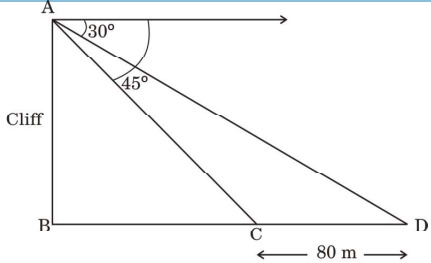
\includegraphics[width=70mm]{cbse-math/figs/boat.edit.jpeg}
        \caption{boat}
        \label{fig:boat.jpeg}
    \end{figure}
    
    Find the height of the cliff.
    
    \hfill\brak{10, 2022}\item The angle of elevation of the top $Q$ of a vertical tower $PQ$ from a point $X$ on the ground is $60\degree$. From a point $Y$, $40$ meters vertically above $X$, the angle of elevation of the top $Q$ of tower $PQ$ is $45\degree$. Find the height of the tower $PQ$ and the distance $PX$. (Use $\sqrt{3} = 1.73$)
    
    \hfill\brak{10, 2022}\item An Aeroplane at an altitude of $200$ meters observes the angles of depression of opposite points on the two banks of a river to be $45\degree$ and $60\degree$. Find the width of the river. (Use $\sqrt{3} = 1.732$)
    
    \hfill\brak{10, 2022}\item From the top of an $8$ meter high building, the angle of elevation of the top of a cable tower is $60\degree$ and the angle of depression of its foot is $45\degree$. Determine the height of the tower. (Take $\sqrt{3} = 1.732$).
    
    \hfill\brak{10, 2022}\item As observed from the top of a lighthouse $60$ meters high from the sea level, the angles of depression of two ships are $45\degree$ and $60\degree$. If one ship is exactly behind the other on the same side of the lighthouse, then find the distance between the two ships. (Use $\sqrt{3} = 1.732$)
    
    \hfill\brak{10, 2022}\item At a point on the level ground, the angle of elevation of the top of a vertical tower is found to be $\alpha$, such that $\tan\alpha = \frac{5}{12}$. On walking $192$ meters towards the tower, the angle of elevation $\beta$ is such that $\tan\beta = \frac{3}{4}$. Find the height of the tower.
    
    \hfill\brak{10, 2022}\item $\tan^{-1}\frac{1}{\sqrt{3}} - \cot^{-1}\frac{-1}{\sqrt{3}}$
    
    \hfill\brak{10, 2022}\item Two angles of a triangle are $\cot^{-1}2$ and $\cot^{-1}3$. The third angle of the triangle is?
    
    \hfill\brak{10, 2022}\item Solve for $x$:
    \begin{align}
        \sin^{-1}(1-x) - 2 \sin^{-1} x = \frac{\pi}{2}
    \end{align}
\hfill\brak{10, 2022}
\item If $2\cos  \theta = \sqrt{3}$ , then find the value of $\theta$
\hfill\brak{10, 2021}\item  In $\triangle ABC$, right-angled at $A$, if $AB=7 cm$ and $AC=24 cm$, then find $\sin B$
and $\tan C$.

\hfill\brak{10, 2021}\item If  $\sin (A+B) = \sqrt{3}/2,
 \sin (A-B) = 1/2,$ Where $0\degree<A+B<90\degree; A>B$, then find the values of $A$ and $B$.

\hfill\brak{10, 2021}\item  Simplify :
\begin{align}
\frac{\sin 30\degree + \tan 45\degree-\cos 60\degree}{\sec 30\degree + \cos 60\degree + \cot 45\degree} 
\end{align}


\hfill\brak{10, 2021}\item Prove that :
\begin{align}
 \sec \theta (1-\sin\theta)(\sec\theta+ \tan\theta)=1
\end{align}

\hfill\brak{10, 2021}\item Prove that :
\begin{align}
\frac{1+\sec A}{\sec A}=\frac{\sin^2 A}{1-\cos A} 
\end{align}

\hfill\brak{10, 2021}\item If  $\tan \theta = 4/3$, find the value 
$\frac{2\sin \theta -3\cos \theta}{2\sin\theta+3\cos\theta}$

\hfill\brak{10, 2021}\item If x=  $a\cos\theta$ and y=$b\sin\theta$, then find the value of   $b^2x^2+a^2y^2$

\hfill\brak{10, 2021}\item Prove that :
\begin{align}
\frac{\tan\theta-\cot\theta}{\sin\theta\cos\theta}=\tan^2\theta-\cot^2\theta 
\end{align}
\hfill\brak{10, 2021}\item Prove that:
\begin{align}
(\sec\theta-\tan\theta)^2 =\frac{1+\sin\theta}{1-\sin\theta}
\end{align}

		\hfill\brak{10, 2021}\item If $3\sin A = 1$, then find the value of $\sec A$.
		\hfill\brak{10, 2021}\item Show that: $\frac{1 + \cot^2{\theta}}{1 + \tan^2{\theta}} = \cot^2{\theta}$.
\hfill\brak{10, 2021}\item Simplify :$${\csc^{2}{60\degree} \sin^{2}{30\degree} - \sec^{2}{60\degree}}$$
	\hfill\brak{10, 2021}\item If $\tan{\theta} + \cot{\theta}$ = $\frac{4 \sqrt{3}}{3}$, then find the value of $\tan^{2}{\theta} + \cot^{2}{\theta}$. 
		\hfill\brak{10, 2021}\item Prove:$$\frac{1}{(\cot A)(\sec A) - \cot A} - \csc A = \csc A - \frac{1}{(\cot A)(\sec A) + \cot A}$$
		\hfill\brak{10, 2021}\item Prove:$$\sin^{6} A + 3\sin^{2} A \cos^{2} A = 1 - \cos^{6}  A$$
		\hfill\brak{10, 2021}\item A man on the top of a vertical tower observes a car moving at a uniform speed coming directly towards it. If it takes $18$ minutes for the angle of depression to change from $30\degree$ to $60\degree$, how soon after this will the car reach the tower ?

		\hfill\brak{10, 2021}\item A girl on a ship standing on a wooden platform, which is $50$ m above water level, observes the angle of elevation of a top of a hill as $30\degree$ and the angle of depression of the base of the hill as $60\degree$. Calculate the distance of the hill from the platform and the height of the hill.
\hfill\brak{10, 2021}
\item Two angles of a triangle are  $\cot^{-1}2$ and $\cot^{-1}3$.The third angle of the
triangle is \rule{30pt}{1pt}

\hfill\brak{12, 2021}\item Prove that $2\tan^{-1}\frac{1}{2} + \tan^{-1}\frac{1}{7} = \tan^{-1}\frac{31}{17}$

\hfill\brak{12, 2021}\item $ \sin \sbrak[\frac{\pi}{3}-\sin^{-1}(\frac{-1}{2})] $ is equal to:

\begin{enumerate}

\item $\frac{1}{2}$
\item $\frac{1}{3}$
\item -1
\item 1

\end{enumerate}

\hfill\brak{12, 2021}\item $ \sin(\tan^{-1}x)$,where $\abs{x} \le 1 $,is equal to:

\begin{enumerate}

\item$\frac{x}{\sqrt{1-x^2}}$
\item$\frac{1}{\sqrt{1-x^2}}$ 
\item$\frac{1}{\sqrt{1+x^2}}$
\item$\frac{x}{\sqrt{1+x^2}}$

\end{enumerate}  

\hfill\brak{12, 2021}\item Simplest form of $ \tan^{-1}(\frac{\sqrt{1+\cos x}+\sqrt{1-\cos x}}{\sqrt{1+\cos x}- \sqrt {1- \cos x}}) , \pi < x < \frac{3\pi}{2}$ is:

\begin{enumerate}

  \item$\frac{\pi}{4} - \frac{x}{2}$
  \item$\frac{3\pi}{2} - \frac{x}{2}$
  \item$-\frac{x}{2}$
  \item${\pi} - \frac{x}{2}$

\end{enumerate}
\hfill\brak{12, 2021}
\item Prove that 
\begin{align*}
    \sin^{-1}\frac{4}{5}+\tan^{-1}\frac{5}{12}+\cos^{-1}\frac{63}{65}=\frac{\pi}{2}
\end{align*}
\hfill\brak{12, 2019}
\item Find the value of $\sin\brak{\cos^{-1}{\frac{4}{5}}+{\tan^{-1}{\frac{2}{3}}}}$.
\hfill\brak{12, 2019}\item Solve for x:
\begin{align*}
\tan^{-1}\brak{x+1}+\tan^{-1}\brak{x-1}=\tan^{-1}\brak{\frac{8}{31}}
\end{align*}
\hfill\brak{12, 2019}\item Prove that :
\begin{align*}
\cos^{-1}\brak{\frac{12}{13}}+\sin^{-1}\brak{\frac{3}{5}}=\sin^{-1} \brak{\frac{56}{65}}
\end{align*}
\hfill\brak{12, 2019}

\item If $\tan^{-1}x-\cot^{-1}x =\tan^{-1}\brak{\frac{1}{ \sqrt3}}, x>0$ ,find the value of $x$ and hence find the value of $\sec^{-1}\left(\dfrac{2}{x}\right)$.

\hfill\brak{12, 2019}\item  If
\begin{align*}
 \sin^{-1} \brak{\dfrac{3}{x}} + \sin^{-1}\brak{\dfrac{4}{x}}=\dfrac{\pi}{2} 
\end{align*}
then find the value of $x$. 

\hfill\brak{12, 2019}\item Find the value of $x$, if $\tan \brak{\sec^{-1}\brak{\frac{1}{x}}} = \sin \brak{\tan^{-1}{2}},x > 0$.
\hfill\brak{12, 2019}

\item  Evaluate:
\begin{align*}
    \frac {\tan 65\degree}  {\cot 25\degree}
\end{align*}

\hfill\brak{10, 2019}\item Express $\brak{{\sin 67\degree}+ {\cos 75\degree}}$ in terms of trigonometric ratios of the angle between $0\degree$ and $45\degree$.

\hfill\brak{10, 2019}\item Prove that :
\begin{align*}
    \brak{\sin \theta+1+\cos \theta} \brak{\sin\theta-1+\cos\theta}.\sec\theta \csc\theta=2
\end{align*}

\hfill\brak{10, 2019}\item Prove that :
\begin{align*}
      \sqrt{\frac{\sec\theta-1}{\sec\theta+1}} + \sqrt{\frac{\sec\theta+1}{\sec\theta-1}} = 2\csc\theta
\end{align*}

\hfill\brak{10, 2019}\item If $\sec\theta + \tan\theta=m$, show that $\frac{m^2-1}{m^2+1} = \sin\theta$.

\hfill\brak{10, 2019}\item Prove that :
\begin{align*}
    2 (\sin^6\theta +\cos^6\theta) - 3 (\sin^4\theta + \cos^4\theta) + 1 = 0
\end{align*}

\hfill\brak{10, 2019}\item Find $A$ and $B$ if $\sin \brak{A + 2B}=\frac{\sqrt{3}}{2}$ and $\cos \brak{A + 4B} = 0$, where $A$ and $B$ are acute angles.





\hfill\brak{10, 2019}\item Evaluate :
 \begin{align*}
	     \sin^{2}{60\degree} + 2\tan{45\degree} - \cos^{2}{30\degree}. 
      \end{align*}

\hfill\brak{10, 2019}\item Evaluate :
\begin{align*}
\left(\frac{3\tan 41\degree}{\cot 90\degree}\right)^2 - \left(\frac{\sin 3\degree \sec 55\degree}{\tan 10\degree \tan 20\degree \tan 60\degree \tan 70\degree \tan 80\degree}\right)^2
\end{align*}

\hfill\brak{10, 2019}\item Prove that :
\begin{align*}
\frac{\tan \theta}{1-\cot \theta} + \frac{\cot \theta}{1- \tan \theta} = 1+ \sec \theta  \csc  \theta   
\end{align*}

\hfill\brak{10, 2019}\item Prove that :
\begin{align*}
    \frac{\sin \theta}{\cot \theta + \csc \theta} = 2 + \frac{\sin \theta}{\cot \theta - \csc \theta}
\end{align*}

\hfill\brak{10, 2019}\item Evaluate :
\begin{align*}
\left(\frac{3\sin 43\degree}{\cos 47\degree}\right)^2 - \frac{\cos 37\degree \csc 53\degree}{\tan 5\degree \tan 25\degree \tan 45\degree \tan 65\degree \tan 85\degree}
\end{align*}


 \hfill\brak{10, 2019}\item If $\sin A = \frac{3}{4}$, calculate $\sec A$.


\hfill\brak{10, 2019}\item If $\tan$ $\alpha$ = ${\frac {5}{12}}$, find the value of $\sec$ $\alpha$.

\hfill\brak{10, 2019}\item $A$, $B$ and $C$ are interior angles of a triangle $ABC$. Show that
\begin{enumerate}
\item  $\sin$ $ \brak{{\frac {B+C}{2}}} = \cos {\frac {A}{2}}$
\item  If $\angle A = 90 \degree$ , then find the value of $\tan \brak{{\frac{B+C}{2}}}$ 
\end{enumerate} 

\hfill\brak{10, 2019}\item If $\tan \brak{A + B} = 1$ and $\tan \brak{A - B} = \frac{1}{\sqrt{3}}$ , $0\degree$ $<$ $A + B$ $<$ $90\degree$, $A > B$, then find the values of $A$ and $B$.

\hfill\brak{10, 2019}\item If $1 + \sin^2 \theta  = 3 \sin \theta \cos \theta$, then prove that $\tan$ $\theta = 1 $ or $\tan$ $\theta = \frac{1}{2}$

\hfill\brak{10, 2019}\item Prove that :
\begin{align*}
\frac{\tan^3 \theta}{1+\tan^2 \theta} + \frac{\cot^3 \theta}{1 + \cot^2 \theta} =  \sec \theta  \csc  \theta - 2 \sin \theta \cos \theta  
\end{align*}


\hfill\brak{10, 2019}\item If $\sin{x} + \cos{y}= 1$ ; $x=30\degree$  and  $y$ is an acute angle, find the value of $y$ .

\hfill\brak{10, 2019}\item Find the value of $\cos {48\degree} - \sin {42\degree}$.

\hfill\brak{10, 2019}\item Prove that :
\begin{align*}
   {\frac{\tan\theta}{1-\tan\theta}} - {\frac{\cot\theta}{1-\cot\theta}}={\frac{\cos\theta+ \sin\theta}{\cos\theta-\sin\theta}}
\end{align*} 

\hfill\brak{10, 2019}\item If ${\cos\theta + \sin\theta} = {\sqrt 2}{\cos\theta}$, show that ${\cos\theta - \sin\theta} = {\sqrt 2}{\sin\theta}$.

\hfill\brak{10, 2019}\item Prove that :
\begin{align*}
    {\frac{(1+\cot\theta+\tan\theta)(\sin\theta-\cos\theta)}{(\sec^3\theta-\csc^3\theta)}} = \sin^2\theta \cos^2\theta
\end{align*}

\hfill\brak{10, 2019}\item Evaluate :
\begin{align*}
    {\frac{\csc^2(90\degree - \theta)-\tan^2\theta)}{2(\cos^2 37\degree + \cos^2 53\degree)}} - {\frac{2\tan^2 30\degree \sec^2 37\degree \cdot \sin^2 53\degree}{\csc^2 63\degree - \tan^2 27\degree}} 
\end{align*}	




  \hfill\brak{10, 2019}\item Prove that \begin{align*} \brak{\sin\theta + \csc\theta}^2 + \brak{\cos\theta + \sec\theta}^2 = 7 + \tan^2\theta + \cot^2\theta\end{align*}.
  \hfill\brak{10, 2019}\item Prove that \begin{align*}\brak{1+\cot A - \csc A} \brak{1 + \tan A +\sec A} = 2 \end{align*}.
  \hfill\brak{10, 2019}\item Prove that \begin{align*} \frac{\sin A-\cos A+1}{\sin A+ \cos A-1} =\frac{1}{\sec A-\tan A}\end{align*}
  \hfill\brak{10, 2019}\item Find $A$ if \begin{align*}\tan 2A = \cot (A-24\degree)\end{align*}
  \hfill\brak{10, 2019}\item Find the value of \begin{align*}(\sin^2 33\degree+ \sin^2 57\degree)\end{align*}
  
  
  \hfill\brak{10, 2019}\item if If $\sec\theta = x + \frac{1}{4x}$, where $x \neq 0$, find $(\sec\theta + \tan\theta)$.
  \hfill\brak{10, 2019}\item prove that \begin{align*} \frac{\tan^2A}{\tan^2 A-1}+\frac{\csc^2 A}{\sec^2 A-\csc^2 A}=\frac{1}{1-2\cos^2 A}\end{align*}
\hfill\brak{10, 2019}

\end{enumerate}
